\documentclass[12pt, a4paper]{article}

% Поддержка русского языка
\usepackage[utf8]{inputenc}
\usepackage[T2A]{fontenc}
\usepackage[russian]{babel}

% Математические пакеты
\usepackage{amsmath, amssymb, mathrsfs, amsthm}

% Работа с графикой
\usepackage{graphicx}
\usepackage{float}
\usepackage{caption}

% Настройка полей
\usepackage[left=2.5cm, right=1.5cm, top=2cm, bottom=2cm]{geometry}

\begin{document}

\begin{titlepage}
    \begin{center}
        \vspace*{5cm}
        \Huge
        \textbf{От теории к практике: Применение методов математической статистики в реальных задачах}
        
        \vspace{1.5cm}
        \Large
        Методы математической статистики в реальном мире
        
        \vfill
        \normalsize
        \today
    \end{center}
\end{titlepage}

\tableofcontents
\newpage

\section{Оценка каузального эффекта: От снижения дисперсии к Double Machine Learning}

\subsection{Формализация задачи контролируемого эксперимента}
В индустрии часто используется термин \textit{A/B-тестирование}, который в математической статистике известен как рандомизированное контролируемое испытание (Randomized Controlled Trial). Пусть у нас есть случайная величина $Y$ (например, траты пользователя, отклик) и бинарный индикатор воздействия $T \in \{0, 1\}$ (где $T=1$ означает применение новой методики). 

Наша цель — оценить средний эффект воздействия (Average Treatment Effect, ATE):
$$\theta = \mathbb{E}[Y \mid T=1] - \mathbb{E}[Y \mid T=0]$$

В идеальном эксперименте $T$ не зависит от характеристик объекта $X$. В этом случае несмещенной оценкой $\theta$ является разность выборочных средних: $\hat{\theta} = \bar{Y}_1 - \bar{Y}_0$. Однако дисперсия этой оценки $\mathbb{V}(\hat{\theta})$ может быть слишком велика для получения статистически значимых выводов на ограниченной выборке. 

Для сужения доверительных интервалов применяется метод \textbf{снижения дисперсии (Variance Reduction)}, использующий ковариату — некую величину $X$, известную до начала эксперимента. Современной модификацией является использование оценки условного математического ожидания, полученной с помощью алгоритмов машинного обучения: $\hat{Y} = \mathbb{E}[Y \mid X]$. Модифицированная случайная величина конструируется как:
$$Y_{adj} = Y - \gamma (\hat{Y} - \mathbb{E}[\hat{Y}])$$
Дисперсия $Y_{adj}$ существенно ниже исходной $\mathbb{V}(Y)$, что позволяет точнее оценить $\theta$.

\subsection{Проблематика: Смещение выборки (Selection Bias)}
На практике идеальная рандомизация часто нарушается. Возникает проблема обсервационных (наблюдательных) данных, где вероятность получить воздействие $T$ зависит от признаков объекта $X$. В статистике $X$ называют \textit{смешивающей переменной} (confounder). 

Если мы применим наивную оценку $\bar{Y}_1 - \bar{Y}_0$ при наличии зависимости между $T$ и $X$, оценка $\hat{\theta}$ будет математически смещенной (Рисунок \ref{fig:dml}). Алгоритмы машинного обучения, обученные напрямую предсказывать $Y$, «впитают» в себя это системное смещение, показывая ложную корреляцию вместо причинно-следственной связи.

\begin{figure}[H]
    \centering
    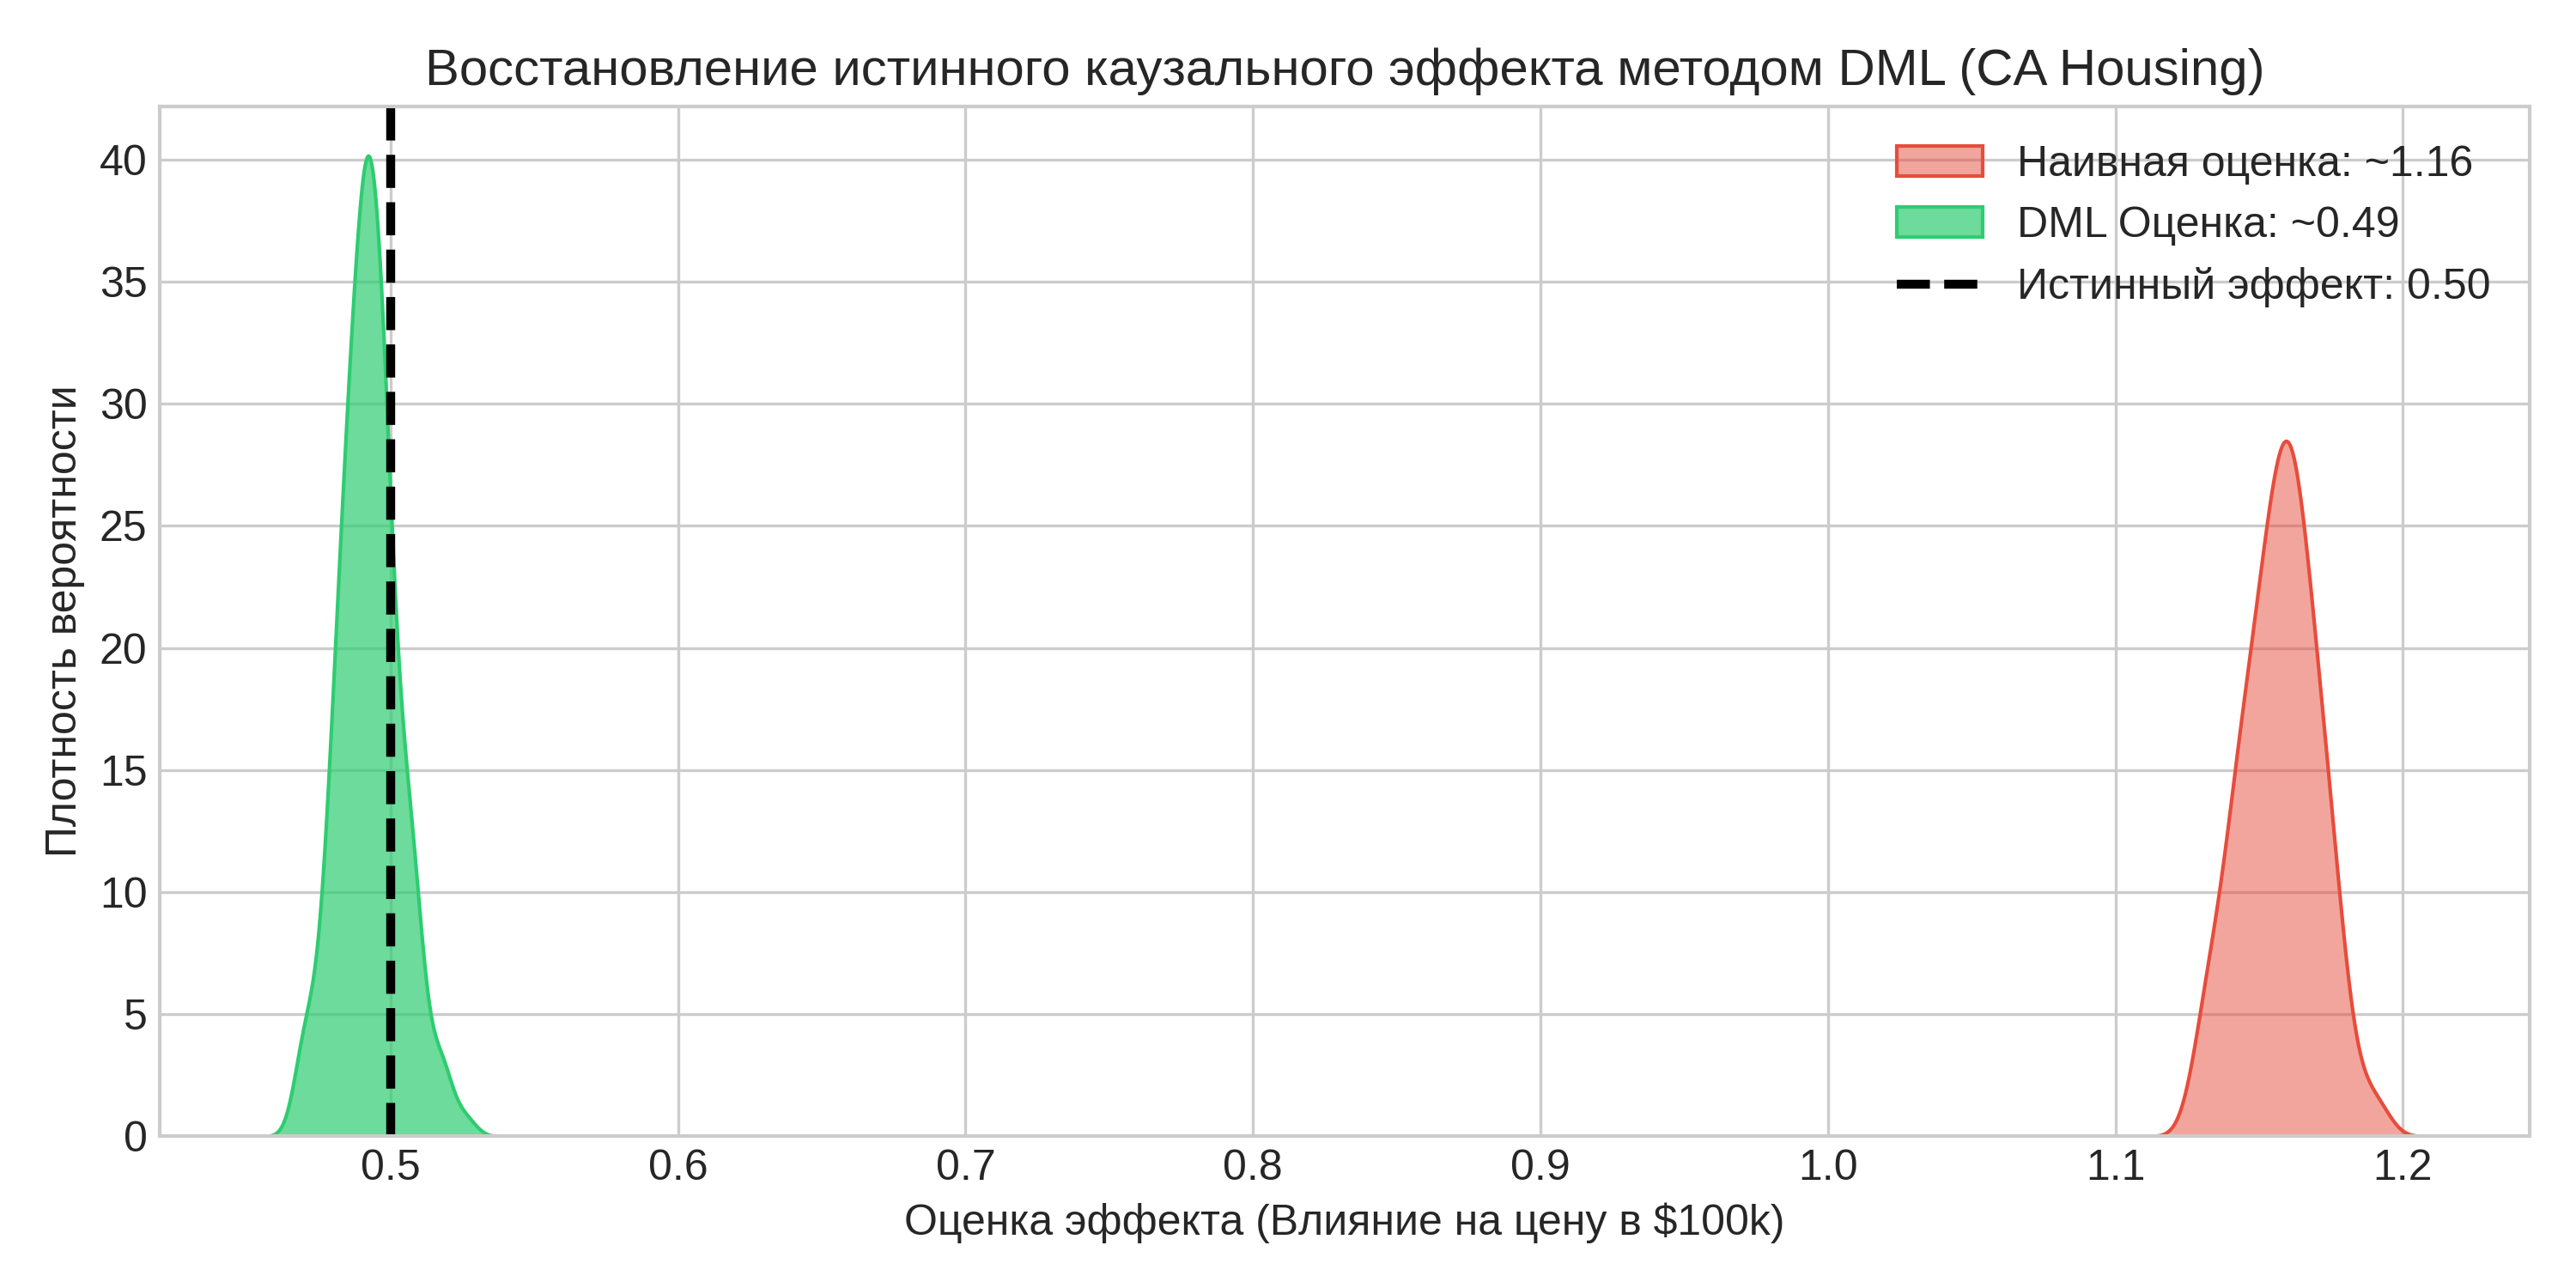
\includegraphics[width=0.9\textwidth]{01_dml_comparison.png}
    \caption{Оценка каузального эффекта (Полусинтетические данные). Наивная оценка вбирает в себя системное смещение (влияние высокого дохода), показывая ложный завышенный эффект. Метод DML успешно изолирует влияние конфаундеров и находит истинный скрытый эффект (черный пунктир).}
    \label{fig:dml}
\end{figure}

\subsection{Решение: Double Machine Learning (DML)}
Для корректной оценки $\theta$ в условиях зависимости $T$ от $X$ применяется метод Double Machine Learning. Предположим частично линейную модель генерации данных:
$$Y = \theta T + g(X) + \epsilon, \quad \mathbb{E}[\epsilon \mid X, T] = 0$$
где $g(X)$ — неизвестная нелинейная функция мешающих факторов. DML использует принцип ортогонализации (теорема Фриша-Во-Ловелла):

\begin{enumerate}
    \item \textbf{Изоляция $Y$ от $X$:} Обучаем алгоритм машинного обучения оценивать $\hat{q}(X) = \mathbb{E}[Y \mid X]$. Вычисляем остатки (шум, не объясненный $X$): $\tilde{Y} = Y - \hat{q}(X)$.
    \item \textbf{Изоляция $T$ от $X$:} Обучаем модель оценивать условную вероятность воздействия $\hat{p}(X) = \mathbb{P}(T=1 \mid X)$. Вычисляем остатки: $\tilde{T} = T - \hat{p}(X)$.
    \item \textbf{Оценка эффекта:} Применяем классический метод наименьших квадратов (МНК) к очищенным остаткам:
    $$\hat{\theta} = \left( \sum_{i=1}^N \tilde{T}_i^2 \right)^{-1} \sum_{i=1}^N \tilde{T}_i \tilde{Y}_i$$
\end{enumerate}
Такой подход нейтрализует влияние мешающих факторов и математически гарантирует асимптотическую нормальность и состоятельность оценки $\hat{\theta}$.

\subsection{Практический кейс: Валидация метода на полусинтетических данных (CA Housing)}
\textbf{Постановка задачи:} При работе с чисто обсервационными данными истинный эффект воздействия (Ground Truth) неизвестен. Для объективной валидации мы используем \textbf{полусинтетический подход}: берем реальные сложные данные для признаков $X$ (доход, гео-локация), но воздействие $T$ моделируем сами. Мы оцениваем эффект установки системы «Умный дом» ($T=1$) на стоимость недвижимости ($Y$).

\textbf{Генерация данных:} 
Используется база \textit{California Housing}. Вероятность установки $T$ жестко зависит от медианного дохода семьи (MedInc) — чем богаче район, тем чаще ставят системы. Истинный заложенный эффект повышения цены от самой системы (ATE) строго равен $0.500$ (в у.е.).

\textbf{Шаги решения и результаты:}
\begin{enumerate}
    \item \textbf{Наивный подход:} Простое сравнение средних дает оценку $\hat{\theta}_{naive} \approx 1.157$. Это классическое смещение выборки: наивная модель приписала системе «Умный дом» эффект богатства самого района, завысив ценность воздействия более чем в два раза.
    \item \textbf{Применение DML:} Модели изолируют влияние дохода и географии. Очищенная оценка DML составляет $\hat{\theta}_{DML} \approx 0.493$.
    \item \textbf{Итог:} Метод DML практически идеально выявил истинный скрытый каузальный эффект ($0.500$), полностью проигнорировав массивный фоновый шум и смещения реальных данных.
\end{enumerate}

\newpage
\section{Оценка неопределенности: От Квантильной регрессии к Conformal Prediction}

\subsection{Формализация задачи анализа экстремальных значений}
В ряде инженерных и бизнес-задач нас интересует не среднее значение случайной величины, а ее границы. Сервис должен гарантировать клиенту, что с вероятностью $95\%$ реальная цена продажи или время ответа не выйдет за указанные рамки:
$$\mathbb{P}(Y \in C(X) \mid X = x) \ge 1 - \alpha$$

Важной особенностью таких систем является \textbf{гетероскедастичность} — условная дисперсия $\mathbb{V}(Y \mid X)$ не постоянна, а возрастает с увеличением $X$. Классический МНК (моделирующий $\mathbb{E}[Y \mid X]$ с постоянной дисперсией) здесь неприменим.

\subsection{Проблематика: Хаотичность границ и физические ограничения}
Наивные подходы используют глобальную ошибку (RMSE) для построения интервалов. На реальных данных с неравномерной дисперсией симметричные интервалы часто упускают сильные выбросы в сложных сегментах и, что более критично, пробивают физические ограничения (например, выдают отрицательную стоимость). 

Кроме того, сложные ансамблевые алгоритмы могут генерировать ступенчатые, хаотичные границы (Рисунок \ref{fig:conformal}). Для отображения пользователям в реальных интерфейсах интервалы должны быть гладкими и физически осмысленными.

\begin{figure}[H]
    \centering
    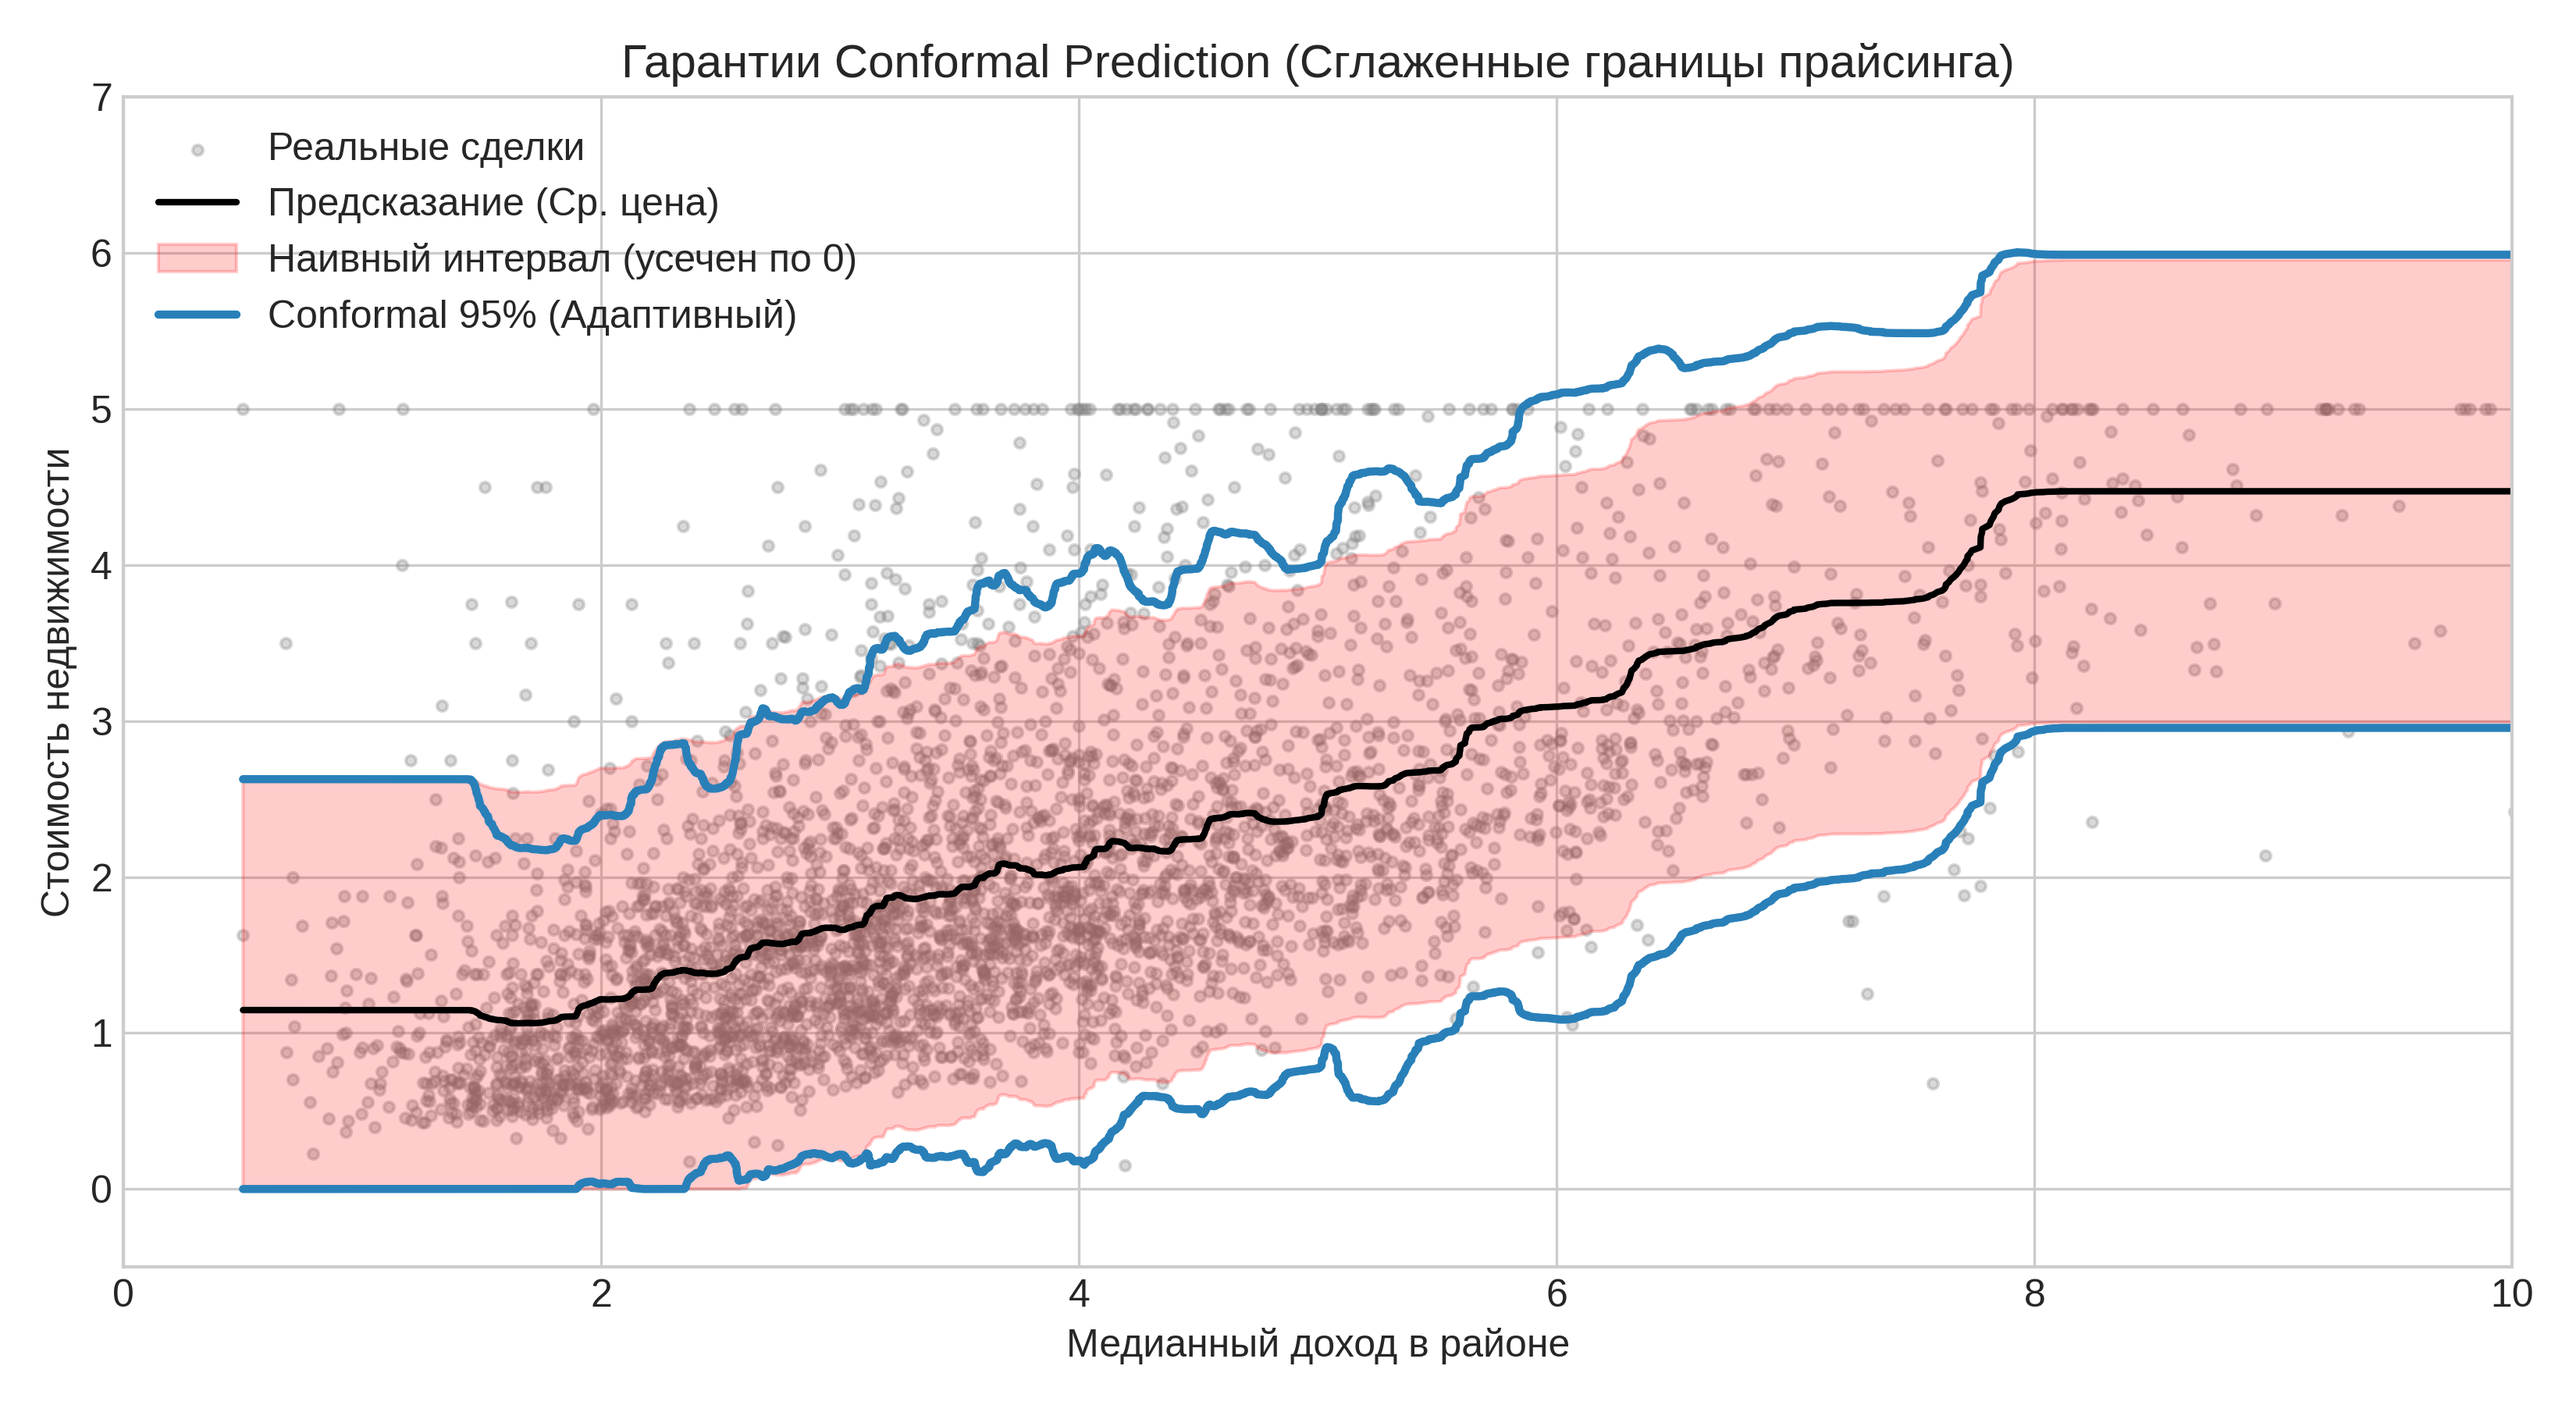
\includegraphics[width=0.9\textwidth]{02_conformal_comparison.png}
    \caption{Прогнозирование стоимости с гладкими границами Conformal Prediction. Наивный интервал проваливается на участках дорогого жилья и жестко усекается нулем внизу. Conformal-интервал адаптивно и гладко расширяется, гарантируя покрытие.}
    \label{fig:conformal}
\end{figure}

\subsection{Решение: Split Conformal Prediction}
Конформные предсказания — это статистический аппарат, который позволяет построить предиктивный интервал $C(X)$ поверх \textit{любой} модели $\hat{\mu}(x)$, гарантируя точное покрытие. Метод опирается на вычисление квантилей нормированных остатков на калибровочной выборке.

Для реальных бизнес-систем вводится условие неотрицательности $max(0, \dots)$, а базовые модели регуляризуются для обеспечения гладкости:
$$C(X_{new}) = \left[\max(0, \hat{\mu}(X_{new}) - \hat{q}\cdot\hat{\sigma}(X_{new})), \, \hat{\mu}(X_{new}) + \hat{q}\cdot\hat{\sigma}(X_{new})\right]$$

\subsection{Практический кейс: Динамическая оценка стоимости недвижимости}
\textbf{Постановка задачи:} Разработка системы оценки стоимости жилья (SLA прайсинга). При росте медианного дохода ($X$) средняя стоимость домов ($Y$) растет, но \textit{драматически} увеличивается разброс цен.

\textbf{Данные:} Датасет \textit{California Housing}.

\textbf{Шаги решения и результаты:}
\begin{enumerate}
    \item \textbf{Наивный подход:} Интервал на базе глобального RMSE дает общее покрытие $92.31\%$. Однако нижняя граница часто становится отрицательной (что физически невозможно), а в сегментах элитного жилья с высокой волатильностью интервал пропускает значительное количество сделок.
    \item \textbf{Conformal Prediction:} Обучаем вспомогательную модель на предсказание дисперсии. Конструируем динамические интервалы со строгим отсечением по нулю и гладкими границами.
    \item \textbf{Итог:} Общее покрытие составило $94.57\%$. Метод адаптивно расширил границы в зоне высоких доходов, надежно выполнив математическую гарантию без нарушения физических ограничений задачи.
\end{enumerate}

\newpage
\section{Калибровка условных вероятностей при дисбалансе классов}

\subsection{Формализация задачи оценки редких событий}
В задачах выявления аномалий (фрод, редкие заболевания) целевая переменная $Y$ бинарна, а классы экстремально несбалансированы: $\mathbb{P}(Y=1) \ll \mathbb{P}(Y=0)$.

Современные алгоритмы машинного обучения возвращают некоторое вещественное число $S(x)$ (score), которое \textbf{не является} истинной условной вероятностью $\mathbb{P}(Y=1 \mid X=x)$. Для принятия оптимальных решений (установки порогов блокировки) баллы необходимо \textbf{откалибровать} — преобразовать в истинные вероятности.

\subsection{Проблематика: Операционная пригодность}
Традиционно качество вероятностей оценивается через Brier Score (среднеквадратичную ошибку вероятностей). Изотоническая регрессия (непараметрический метод) идеально минимизирует эту метрику. Однако при экстремальном дисбалансе (доли процента позитивного класса) данных в области высоких вероятностей исчезающе мало. 

В результате изотоническая регрессия переобучается на локальный шум и "схлопывает" непрерывные оценки в несколько крупных кластеров-ступеней (Рисунок \ref{fig:calibration}). Модель минимизирует Brier Score, но \textit{полностью теряет способность ранжировать объекты} внутри этих ступеней, что делает ее бесполезной для бизнеса.

\begin{figure}[H]
    \centering
    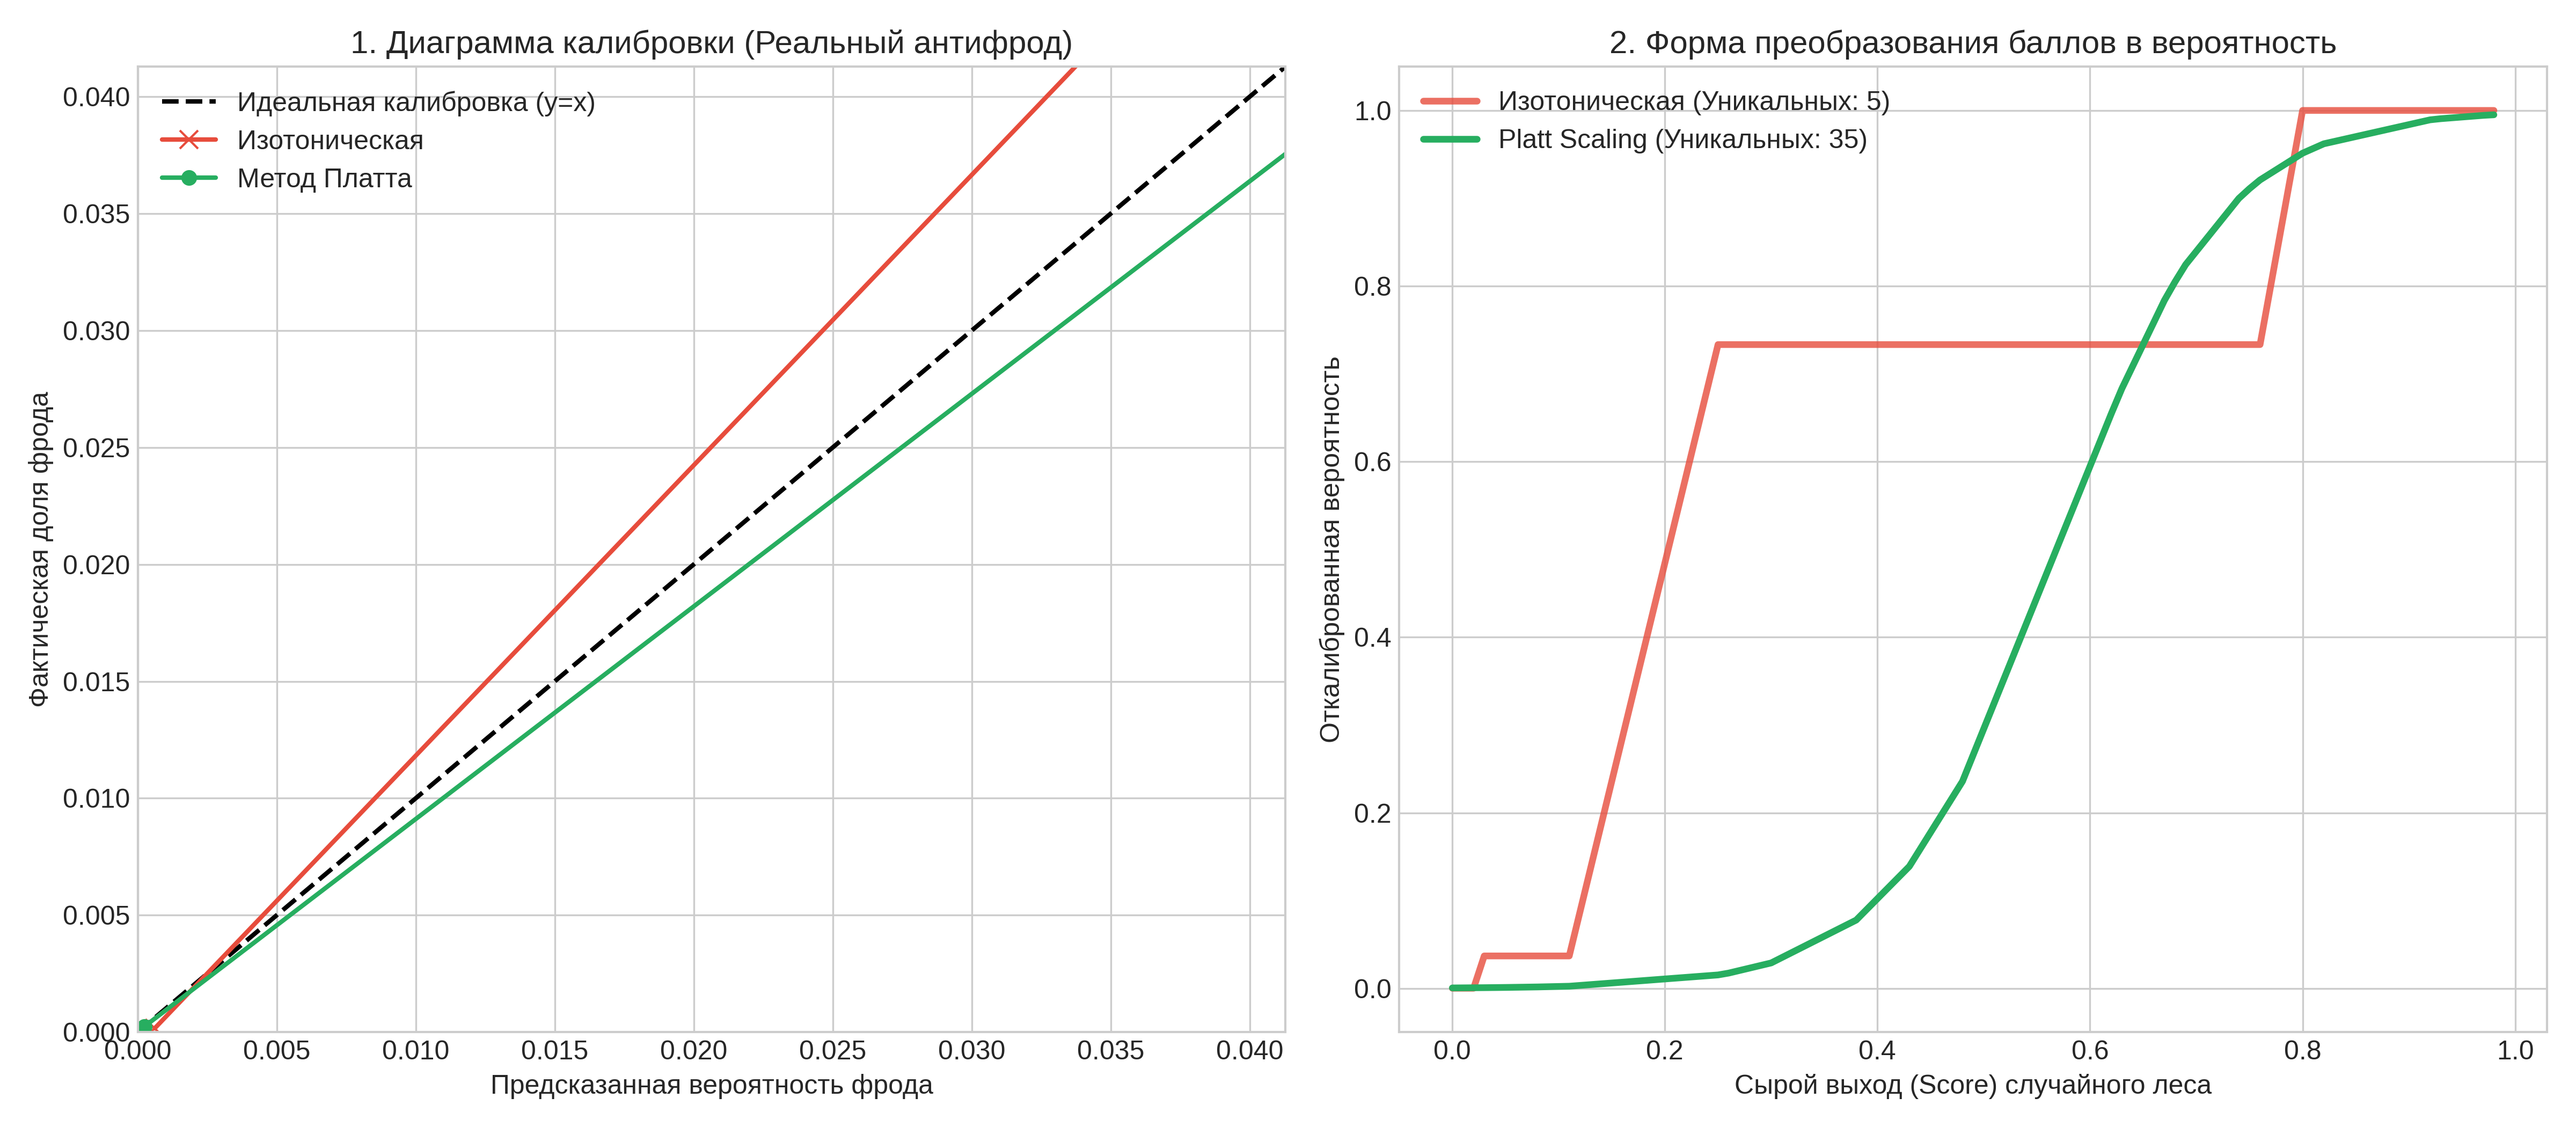
\includegraphics[width=0.9\textwidth]{03_calibration_imbalance.png}
    \caption{Диаграмма калибровки на реальных транзакциях. Изотоническая регрессия превращает баллы в "ступеньки" из-за дисбаланса. Параметрический метод Платта (зеленая линия) сохраняет гладкость и высокую разрешающую способность, несмотря на небольшое отставание по Brier Score.}
    \label{fig:calibration}
\end{figure}

\subsection{Решение: Параметрическая калибровка}
В условиях дефицита объектов миноритарного класса принято переходить к жестким параметрическим семействам. Метод Платта предполагает логистическую связь:
$$\mathbb{P}(Y=1 \mid S) = \frac{1}{1 + \exp\left(- (A \cdot S + B)\right)}$$
Коэффициенты $A$ и $B$ находятся методом максимального правдоподобия. Жесткая форма кривой заставляет ее оставаться гладкой, игнорируя локальный шум и сохраняя уникальность оценок каждого объекта.

\subsection{Практический кейс: Выявление мошеннических банковских транзакций}
\textbf{Постановка задачи:} Система должна выдавать точные вероятности мошенничества для принятия решения о блокировке карты.

\textbf{Данные:} Реальный датасет \textit{Credit Card Fraud Detection} с экстремальным дисбалансом ($0.17\%$ фродовых операций).

\textbf{Шаги решения и результаты:}
\begin{enumerate}
    \item \textbf{Сырая модель:} Деревья решений "сжимают" предсказания. Значение Brier Score сырой модели составляет $\approx 0.00089$.
    \item \textbf{Изотоническая регрессия:} Как и ожидается математически, непараметрический подход выдал лучшую метрику Brier Score ($\approx 0.00068$). \textbf{Но ценой операционной пригодности}: алгоритм сжал сотни тысяч транзакций всего в $5$ уникальных уровней вероятности. Антифрод-система лишилась возможности выявлять градации риска среди клиентов, попавших в один кластер.
    \item \textbf{Метод Платта (Platt Scaling):} Логистическая функция показала Brier Score чуть хуже ($\approx 0.00082$). Однако она сохранила $35$ уникальных оценок риска. Эта незначительная потеря в тысячных долях Brier Score с лихвой окупается сохранением строгой монотонности, позволяя бизнесу выстраивать детальный рейтинговый список подозрительных операций.
\end{enumerate}

\end{document}